\documentclass{article}
\usepackage{graphicx}
\usepackage{listings}
\usepackage{color}
\usepackage[paperwidth=21cm, paperheight=29.7cm]{geometry}
\geometry{paperwidth=21cm, paperheight=29.7cm, tmargin=1.5cm, bmargin=1.5cm,
lmargin=2cm, rmargin=2cm}
\usepackage{tabularx}
\usepackage{tabulary}
\usepackage{tabu}
\usepackage{mathtools}
\usepackage{pgfplots}
\pgfplotsset{compat=newest}
\usepgfplotslibrary{units}
\usepackage{pgfplotstable}
\usepackage{tikz}
\usepackage{filecontents}
\usepackage{csvsimple}
\usepackage{caption}
\usepackage{subcaption}
\usepackage{hyperref}
\usepackage{mathtools}
\usepackage[T1]{fontenc}
\usepackage{colortbl}
\usepackage{makecell}

\definecolor{dkgreen}{rgb}{0,0.6,0}
\definecolor{gray}{rgb}{0.5,0.5,0.5}
\definecolor{mauve}{rgb}{0.58,0,0.82}

\lstset{frame=tb,
  language=C,
  aboveskip=3mm,
  belowskip=3mm,
  showstringspaces=false,
  columns=flexible,
  basicstyle={\small\ttfamily},
  numbers=none,
  numberstyle=\tiny\color{gray},
  keywordstyle=\color{blue},
  commentstyle=\color{dkgreen},
  stringstyle=\color{mauve},
  breaklines=true,
  breakatwhitespace=true,
  tabsize=3
}

\title{Bilinear interpolation algorithm optimalization\\
        with AVX vectorization unit}
\author{
        Jakub Pružinec
        \\
        email: j.pruzinec@gmail.com, university email: xpruzi02@fit.vut.cz
        \\
        Brno University of Technology, Faculty of Information Technologies
        \\
        }
\date{14.12.2018}
\begin{document}
\maketitle

\abstract
{
Resizing is one of the most frequently used image operations and therefore comes in many algorithm
variations. The algorithms are designed to fulfill different criteria. Resizing algorithm is
part of greater project primary focused on collection of media file metadata where execution
speed is major consideration. Bilinear interpolation resizing is one of algorithms that are
designed to be fast. In this project I design, implement and test sequential and parallel bilinear
interpolation algorithm and then I consider its suitability for parallelism and image metadata
gathering.
}
\section{Introduction}
\subsection{Media info gatherer}
Metadata info gatherer is a project focused on media file metadata collecting. Exported
metadata is to be further processed in order to decet duplicity of images, videos,
audio files etc. File system metadata is easy to obtain and is good for duplicity hints,
however it is volatile and unreliable. For these reasons it is often necessary to inspect
file content and produce fingerprint metadata.
\subsection{Perceptual hashes}
One option to identify file content is to produce its cryptic hashes like SHA256 or MD5, but
they are expensive in terms on computation time. Also a minor change in file content is
reflected by major change in its cryptic hash. All of these inconveniences can be avoided
with perceptual hashes when it comes to image processing. Perceptual hashes are hashes
that represent images in a way that their similarity can be determined based on them.
One of computationally inexpensive perceptual hashes is average hash.
\subsection{Average hash}
Average hash is similar to low pass filter output when images are considered signals.
Images are resized to 8x8 to filter out small frequencies effectively ignoring image details.
Then they are converted to greyscale and to black and white afterwards. All of 64 pixels
produced this way are either black or white. Every pixel can represented with a binary
value, 0 for black and 1 for white, creating a 8 byte average hash.
\begin{figure}[h!]
    \centering
    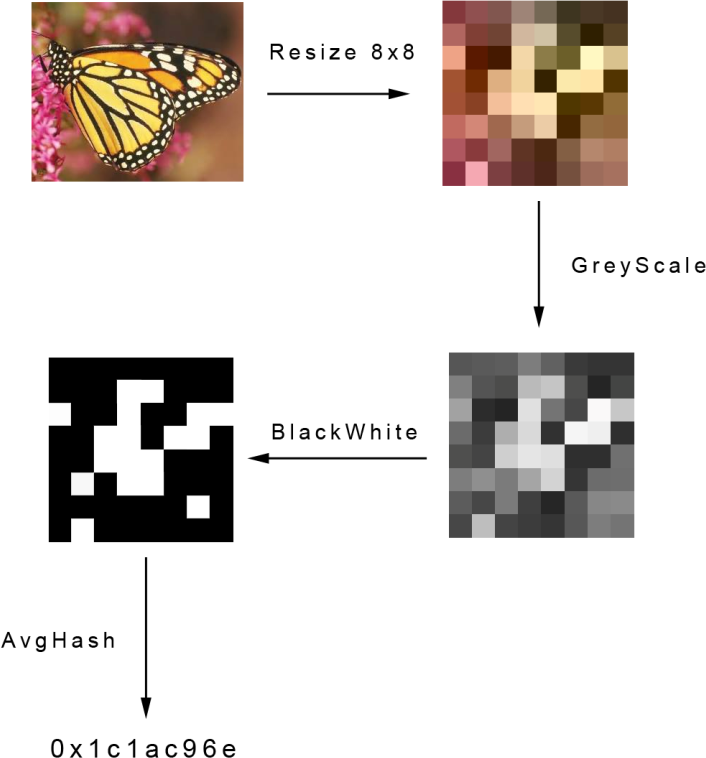
\includegraphics[width=6cm]{avg_hash.png}
    \caption{Average hash computation block schema}
    \label{fig:average hash computation}
\end{figure}
\subsection{Similarity matric}
Similarity of two images is determined by the number of similar pixels. Taking into cosidaration
that every bit of average hash represents a pixel color the similarity of images can be
expressed as Hamming distance of their average hashes. Images whose average hashes Hamming
disntace is 3 or less are considered similar.
\subsection{Bilinear interpolation}
In process of average hash computation images are resized. In
\href{https://archive.org/download/Lectures_on_Image_Processing/EECE_4353_15_Resampling.pdf}
{bilinear interpolation algorithm} every pixel in new image $P'$ is an interpolation of four
pixels $P_1, P_2, P_3, P_4$ from original image. Choice of interpolated pixels is dependant on
image horizontal and vertical scale.
\begin{figure}[h!]
    \centering
    \includegraphics[width=10cm]{bilinear_interpolation.png}
    \caption{Bilinear interpolation}
    \label{fig:bilinear interpolation}
\end{figure}
\section{Design}
\subsection{Bitmap parser}
Bitmap format is commonly used format for image files. To process image content it needs to be
converted to internal representation first. Images are parsed to structures consisting of
image dimensions and three color channel byte arrays. Channel arrays are allocated as continuous
memory chunk to maximize the chance of loading them in a single cache line.
\subsection{Na\"ive bilinear interpolation algorithm}
Na\"ive bilinear interpolation resizing is depicted in following psedo code.
\begin{lstlisting}
calculate horizontal and vertical scales sr, sc
for (rNew in newHeight)
    for (cNew in newWidth)
        calculate interpolated pixels coordinates
        bounds check
        calculate deltas
        for (every channel)
            read 4 pixles and calculate their weights
            multiply pixel colors with weights
        calculate new channel values as sum of four previous results
        store new pixel
\end{lstlisting}
\newpage
\subsection{Sequential bilinear interpolation algorithm}
Removing unnecessary calculations from na\"ive algorithm leads to significant efficiency increase.
Sequential bilinear interpolation algorithm has the following modifications:
\begin{itemize}
    \item interpolated horizontal pixels coordinates calculated in outer loop
    \item interpolated pixels coordinates are incremented in every iteration to avoid multiplication
    \item horizontal delta calculated in outer loop
    \item horizontal fragments of weight formulas are calculated in outer loop
    \item weights are precalculated for all channels only once
\end{itemize}
\begin{lstlisting}
calculate horizontal and vertical scales sr, sc
for (rNew in newHeight)
    increment rf with horizontal scale
    calculate horizontal coordinates of interpolated pixels
    calculate horizontal delta
    calculate horizontal fragments of weight formulas
    for (cNew in newWidth)
        increment cf with vertical scale
        bounds check
        calculate vertical coordinates of interpolated pixels
        calculate vertical delta
        calculate weights
        for (every channel)
            multiply pixel colors with weights
        calculate new channel values as a sum of four previous results
        store new pixel
\end{lstlisting}
\subsection{Parallel bilinear interpolation algorithm}
Since most of operations in inner loop are same for all of image pixels, the pixels are processed
parallely. Vector can contain 8 pixel values, thus 8 pixels are processed simultaneously. To minimize
parallel processing overhead the following algorithm substitutions are designed:
\begin{itemize}
    \item incrementation of $cf$ $\rightarrow$ vector of indices $V_i = (0.0, 1.0, ..., 7.0)$ is
            multiplied with horizontal scale vector $V_{\text{sc}} = (sc, sc, ..., sc)$ then in
            every inner iteration vector $V_i$ is incremented with vector
            $V_{\text{8sc}} = (8sc, 8sc, ..., 8sc)$
    \item inner loop $\rightarrow$ the inner loop is iterated with 8 pixel step and all pixels are
            processed parallely. Remaining pixels are processed sequentialy in separate loop
            afterwards.
    \item bounds check $\rightarrow$ bounds check is done by sequence of vector masking and vector
            logical operations
\end{itemize}
\begin{lstlisting}
calculate horizontal and vertical scales sr, sc
for (rNew in newHeight)
    increment rf with horizontal scale
    calculate horizontal coordinates of interpolated pixels
    calculate horizontal delta
    calculate horizontal fragment of weight formulas
    assign cf vector with mutiplication of index and sc vector
    for (8cNew pixels in newWidth)
        mask out values exceeding bounds
        calculate vector of vertical coordinates of interpolated pixels
        calculate vector of vertical deltas
        calculate vector of weights
        for (every channel)
            read 8 values sequentialy
            multiply pixel colors vector with weights
        calculate 8 new channel values as a sum of four previous vector results
        store new pixels
        increment cf vector with 8sc vector
\end{lstlisting}
The major bottle neck here is that interpolated pixel coordinates need to be computed in every
iteration and thus \textbf{interpolated pixel colors have to be read from memory sequentialy}.
\newpage
\section{Implementation}
\subsection{Compilation and execution}
To build demonstration project execute the following commad
\begin{lstlisting}
make
\end{lstlisting}
Program synopsis
\begin{lstlisting}
./image-info <imagefile1> <imagefile2>
./image-info_avx <imagefile1> <imagefile2>
\end{lstlisting}
\textit{Image-info} parses two 24bit color depth Bitmap files, prints their average hashes and
determines their similarity.
\subsection{Resizing codes}
Sequential code is written in C language and can be found in \textit{./src/image\_resize.c}.
\\
Parallel code is written in C language with AVX1 SIMD, single instruction multiple data, intrinsic
functions and can be found in \textit{./src/image\_resize\_avx.c}
\section{Performance analysis}
In order to estimate algorithm efficiency the \textit{main()} function is altered to resize
image 1000 times. When measuring execution time image parsing time is neglected. Results are
compared to previous attempts of
\href{https://sites.google.com/site/zhangxujienet/streaming-simd-extensions-sse}
{bilinear interpolation algorithm optimization by Xujie Zhang}. Note that testing hardware,
Intel Core i5 2540M, is \href{http://cpuboss.com/cpus/Intel-Core-i5-2540M-vs-AMD-FX-8350}
{comparable} with the referenced one, AMD FX 8350.
\begin{table}[h!]
    \centering
    \begin{tabu}{*{3}{|c}|}
        \hline
        \cellcolor{yellow!30}\thead{Optimization method} & \cellcolor{yellow!30}\thead{Time/ms} &
        \cellcolor{yellow!30}\thead{Image info\\efficiency improvement}
        \\\hline
        \makecell{Zhang's sequential\\code} & \makecell{11.34} & \makecell{-}
        \\\hline
        \makecell{Zhang's SIMD\\code} & 6.93 & \makecell{-}
        \\\hline
        \makecell{Image-info\\sequential code} & \makecell{4.38} & \makecell{159\%}
        \\\hline
        \makecell{Image-info\\SIMD code} & \makecell{5.8} & \makecell{19\%}
        \\\hline
    \end{tabu}
    \caption{Performance results}
\end{table}
\section{Conclusion}
Despite outperforming both, sequential and parallel, previous implementations of algorithm it is
necessary to consider the suitability of SIMD approach in bilinear interpolation. SIMD version of
algorithm has a drastic decrease in performance. This is due to inevitability of sequential
memory accesing and the fact that parallelism of few operations benefit is too small to cover
overhead that use of SIMD instructions brings.

Further, it is worth to note that bilinear interpolation might not be the best choice when it
comes to average hashes. When downscaling images with bilinear interpolation only a fraction of
pixels is taken into account. This is particularly inconvenient when comparing images with noise.
Noise can be significantly reflected in downscaled image if it overlaps with pixels from original
image that are not ignored. If this is a concern, then e.g box sampling might be a better choice.
\section{Resources}
\href{https://sites.google.com/site/zhangxujienet/streaming-simd-extensions-sse}
{Bilinear interpolation algorithm optimization by Xujie Zhang}
\\
\href{https://archive.org/download/Lectures_on_Image_Processing/EECE_4353_15_Resampling.pdf}
{Digital image processing by Richard Alan Peter}


\end{document}